\documentclass[conference]{IEEEtran}
\IEEEoverridecommandlockouts
% The preceding line is only needed to identify funding in the first footnote. If that is unneeded, please comment it out.
\usepackage{cite}
\usepackage{amsmath,amssymb,amsfonts}
\usepackage{algorithmic}
\usepackage{graphicx}
\usepackage{textcomp}
\usepackage{tabularx}
\usepackage{xcolor}
\usepackage{wrapfig}
\usepackage{hyperref}
\usepackage{subfig}
\def\BibTeX{{\rm B\kern-.05em{\sc i\kern-.025em b}\kern-.08emhttps://www.overleaf.com/9135752949xhrzxszstcwx
    T\kern-.1667em\lower.7ex\hbox{E}\kern-.125emX}}
\begin{document}

\title{To Deny Or Not To Deny: Predicting Case Status For Visa Petitions\\}
\author{\IEEEauthorblockN{Dweepa Honnavalli}
\IEEEauthorblockA{
\textit{Dept. Of Computer Science}\\
\textit{PES University} \\
01FB16ECS138
}
\and
\IEEEauthorblockN{Ishita Bhandari}
\IEEEauthorblockA{
\textit{Dept. Of Computer Science}\\
\textit{PES University} \\
01FB16ECS143
}
\and
\IEEEauthorblockN{Kavya Varma}
\IEEEauthorblockA{
\textit{Dept. Of Computer Science}\\
\textit{PES University} \\
01FB16ECS162
}
}

\maketitle
\begin{abstract}
The paper aims to predict whether a visa applicant to the United States of America is certified or denied a visa. The work presented 
determines  how  visa  status  outcome  of  three  most  applied-to visa-categories (H1-B, L1, and F1) are influenced by attributes of
user application metadata. The model uses different approaches to  predict  the  outcome  of  the  different  classes  of  visas.  The
results of this paper can be utilized by visa aspirants to predict the  outcome  of  their  petition  and  get  recommended  ways  of
maximizing  success  of  acceptance. We developed a prediction model which trains on historical data of the same application domain (i.e based on which visa the applicant has applied to) and uses machine learning classifiers  to  predict  the  outcome  of  visa  petitions. The  allotment  of  most these  visas, like H1-B for example,  is  said  to  be  a  lottery  system not  depending  on  any  specific  criteria.  Thus,  a  foreign  national is  not  guaranteed  selection  for  an  H1B  visa  merely  because  they  fulfill  all  the  qualifying  criteria.  This  work  aims  to  use machine  learning  on  known  factors  to  make  predictions  under this  uncertainty,  with  accuracy  better  than  that  achieved  using the  prior  probability.
\end{abstract}

\begin{IEEEkeywords}
visa, status, prediction, classification,
regression, model, analysis
\end{IEEEkeywords}

\section{Introduction}
The current political and socio-economic status of the world makes entering countries like the United States of America, arduous work. Granting visas to foreign nationals has been restricted. It is hard to predict whether a visa application will be accepted or rejected, especially as different visas are applied for different reasons and have different metadata and criteria for acceptance or rejection.

The H-1B is an employment-based, non-immigrant
visa category for temporary foreign workers in the
United States. For a foreign national to apply for H1-B
visa, a US employer must offer a job and petition for
H-1B visa with the US immigration department. This
is the most common visa status applied for and held
by international students once they complete college. H-1B visa class is very industry relevant
and many individuals and companies rely heavily on
this yearly allotment.

The L-1 visa facilitates the temporary transfer of foreign worker in the managerial, executive or specialized knowledge category to the U.S. to continue employment with an office of the same employer, its parent, branch, subsidiary or affiliate. This is also one of the most common visa application type.  It is a non-immigrant visa, and is valid for a relatively short amount of time, from three months to five years, based on a reciprocity schedule. With extensions, the maximum stay is seven years.

An F1 visa is a nonimmigrant visa for those wishing to study in the U.S. You must file an F1 visa application if you plan on entering the US to attend a university or college, high school, private elementary school, seminary, conservatory, language training program, or other academic institution.

Performing data analytics and predictive analytics on datasets such as these which include a lot of human intuition and decision making to arrive at the outcome, presents some interesting results. These results can be used to understand the less understood part of decision making and the visa process as a whole. Applicants can get more insight on their application and can try to maximise their success based on the results gleaned.

\textit{
There a few models out there, which can predict the outcomes of visa status with decent accuracy but currently there is very little work being done in understanding the effect and impact of each feature. In our project, we aim not only to create a working classifier model, but also use the information gleaned from the models to gain better insight into the features that hold bearing in the decision making.}

\section{Literature Review}
'Understanding factors that influence L1-visa outcomes in US' by Nihar Dalmia, Meghana Murthy and Nianthrini Vivekanandan \cite{berk}attempts to understand the various influencers in the outcome of a L1 visa application by viewing the problem from the perspective of the employer i.e. they endeavor to present the factors that influence the outcome of an application thus allowing employers to recruit the most appropriate candidate to offer a job through an L1 visa. The authors combined the visa application dataset with other relevant datasets like religious diversity of the country of origin, rise of GDP of country of origin, education rate of employer state etc, allowing for a more informed model. Their approach starts off with understanding the extent to which a feature affects the outcome, by performing significance tests. They then construct models for Decision Trees, Logistic Regression, Random Forest, ML Perceptron, Gradient Boosting, Naive Bayes. Two models are created for each approach, one with down sampling and another with SMOTE (Synthetic Minority Oversampling Technique).

'Predicting Case Status of H-1B Visa Petitions in US' by Induja Sreekanthan, Jahnavi Singhal, Prahal Arora and Rahul Dubey attempts to discover how the outcome of a visa application is influenced by attributes of a users application. Features were chosen for prediction by visualising the variations and relations between features. Positive correlation values between acceptance rate and the attribute indicate it might be a good feature.

'Predicting the Outcome of H-1B Visa Applications' by Beliz Gunel and Onur Cezmi Mutlu \cite{stanford}aims to predict the outcome of H-1B visa applications that are filed by many high-skilled foreign nationals every year by treating it mainly as a classification problem. During the stage of pre-processing, they attempt to weed out applications belonging to certain minority classes either as they are small in number or because they may be incorrect. New features that were considered positive addition were generated such as company success rate. The final datasets on which the classification algorithms are a combination of the original features along with the newly generated ones. Classification algorithms like Logistic Regression, Naive Bayes, Support Vector Machines and Neural Network with L2 regularization were used to create models. They preferred stochastic gradient descent over batch gradient descent due to the size of the dataset. They also performed different types of regularization such as l1,l2 and ElasticNet (combination of l1 and l2) on the model to increase the test accuracy. 

'Predictive Modeling of the Journey from H-1B to Permanent US Work Visa' by Shibbir Khan creates a model that predicts the likelihood of a person with an H-1B visa being given a permanent US work visa. The majority of the paper details the various visual exploratory analysis undertaken in an attempt to understand patterns in the dataset. Plots of acceptance on the basis of job title, country of origin, wage offer, degree of education etc have been made. As the dataset mostly consists of categorical values, probabilistic methods were used, such as Gaussian Naive Bayes, Logistic Regression, Gradient Boosted Classifier, Tree Ensemble Learner Classifier. Then the feature importance graph shows the feature importance of the variables in the model and lists out the attributes most influential to the outcome.

'H-1B Visa Data Analysis and Prediction by using K-Means Clustering and Decision Tree Algorithms' by Renchi Liu and Jinglin Li \cite{github} attempts to apply machine learning algorithms to the dataset containing application details of H-1B visas to ascertain which will be accepted. Along with predictive analysis, they also propose to answer trend related questions like what are the top companies that have apply to the H-1B for employees, what is the trend in the total number of H-1B application is, what is the top popular job title and worksites for H-1B visa holders, what is the salary mean values of respective job titles etc. The predictive models created were using the techniques decision trees and K-means clustering. 

\section{Problem statement}
Every year, thousands of companies submit visa applications to the Department of Labor on behalf of foreign workers the companies are trying to hire. These applications differ in many ways: the type of job being applied for, the company sponsoring the application, the location where the foreign worker will be based, educational qualification requirements for the job, how much the job pays, etc. All of these features have a bearing on the outcome of the application. Sometimes the actual outcome of these application can be known only after a long time. In such scenarios, it might be imperative for both the seeker of the visa application and to the employer applying for the visa.

Whether a visa application is accepted or rejected is decided by a variety of factors. A significant aspect of our project aims at understanding these underlying factors, ascertain the degree to which the outcome is based on these factors. This would involve generating plots of the variety of features at our disposal and analyzing the influence of the feature on the outcome. Gaining a clear understanding of the factors that have a bearing on the outcome can be useful to applicants, companies and even data analysts who wish to detect patterns and trends in the data.

The primary aspect of this project is to generate predictive models for the three visa type, H-1B, L-1 and F1 that can analyze a user's application and predict whether it will be rejected or accepted. Through this project we attempt to clean and process the available dataset, create predictive models and use metrics like confusion matrices and ROC to analyze the outcomes of these models. The outcome of this project must include a careful analysis of the predictive models along with their merits and demerits.
\section{ Proposed system}


\subsection{\textbf{Block Diagram}}
\begin{center}
\begin{figure}[h]
\centering
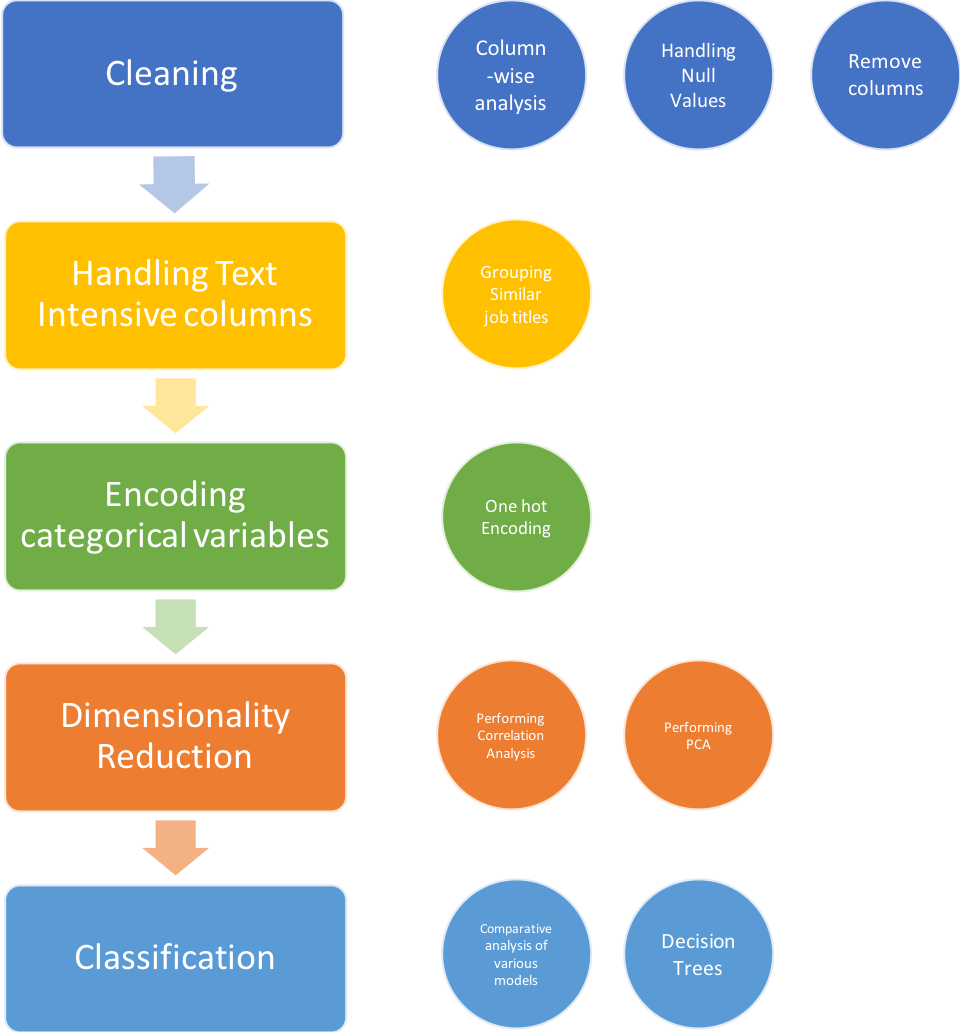
\includegraphics[width=0.35\textwidth]{blockdiagram.png}
\caption{Block Diagram}
\label{fig:mesh1}
\end{figure}
\end{center}


\subsection{\textbf{Dataset}}
The dataset under consideration consists of information about visa applicants to the United States of America.\cite{dataset} \\
There are a 154 columns containing attributes of the applicants like country of citizenship, employer details, educational qualification, job profile etc. Majority of the columns are categorical or non-numeric in nature and hence cannot be consumed by a mathematical model in this unrefined state.\\  
Almost every column has a percentage of its values to be 'NaN' which either indicate that the attribute might not have been applicable to the person of interest or the data might not have been collected in the first place.\\
The number of columns have to be brought down to an actionable amount of information without losing important information.
\\
\subsection{\textbf{Cleaning}
}Preprocessing is a very important step in the grand scheme of events. It is consequential, bearing great significance in the steps to come.
\\
\subsubsection{\textbf{Handling Null Values}}
Null or NaN values signify missing or irrelevant data. There are several approaches to handling these values like discarding them, imputing them or assigning a value that is the average of the column to them.

Below is a table representing the number of columns containing a given percentage (or more)  of their values as NaN.
\\
\begin{center}
\captionof{table}{Null Values in Columns} \label{tab:title}
  \begin{tabularx}{0.45\textwidth}{| l | r| }
  \hline
     \shortstack{\\Percentage of Null values\\ in the column} &
    \shortstack{\\Number of columns \\ exhibiting this behaviour}\\ \hline
    99\% or more & 7 \\ 
    90\% or more & 32 \\
    50\% or more & 84 \\
    25\% or more & 137 \\\hline
  \end{tabularx}
\end{center}

The above table indicates that 50\% (or more) values of 84 columns is NaN. It is illogical to impute so many values for a column, which is the reason these columns are dropped entirely.

Another problem was that the dataset had 374362 rows. Processing this large number of entries is not a practical approach. We eliminated rows based on the number of null entries in it. We calculated the number of NaN entries in each row and removed all the rows with more than 3 NaN values. This cut down our dataset to 158883 rows.

The initial approach to impute the null values present in our data base was to use a KNN model to find the closest neighbours of the row containing the missing value and use these neighbours to determine the value that should be imputed. This approach failed as the memory requirement to perform KNN on a database as large as ours is too high. While this is the approach that bears the most logical merit, it had to be eliminated due to its impracticality.

The next approach attempted was mean value insertion where in we found the mean values of each of the columns and inserted those in the missing cells.
\\
\subsubsection{\textbf{Visualization}}
Visualization is done to understand the dataset better. Some of the useful visualizations are listed below.
\paragraph{\textbf{Most Certified countries: }}
\begin{center}
\begin{figure}[h]
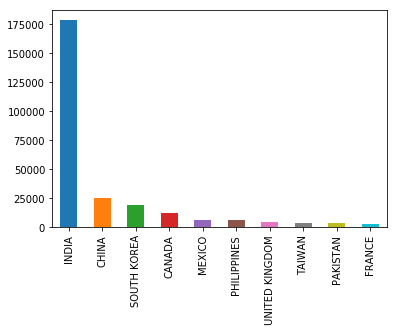
\includegraphics[width=0.45\textwidth]{country.png}
\caption{Most certified countries}
\label{fig:mesh1}
\end{figure}
\end{center}
Analysis and visualization of the 'country\_of\_citizenship field' showed us that the most number of delegates who got 'Certified' visa status were from India during the time period of 2007 to 2016.
\paragraph{\textbf{Growth Rates: }}
The above graph shows the growth of the number of accepted delegates during the period of 2007 to 2016 for each of the classes of admission.
\begin{center}
\begin{figure}[h]
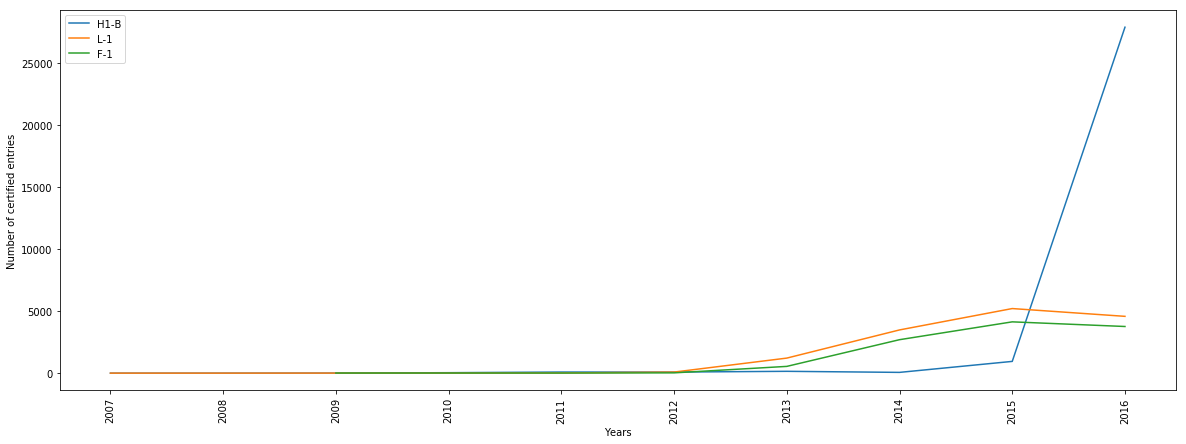
\includegraphics[width=0.45\textwidth]{growth.png}
\caption{Growth rates}
\label{fig:mesh1}
\end{figure}
\end{center} 
\paragraph{\textbf{Most Certified Agent Firms: }}
Analysis of agent\_firm\_name showed that there are some firms that have dominated this market and done it well like Fragomen Del Rey Bernsen & Loewy.
\begin{center}
\begin{figure}[h]
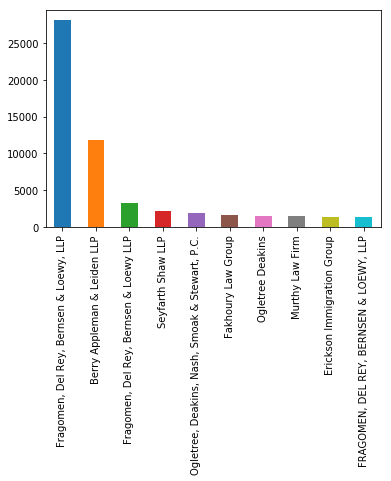
\includegraphics[width=0.45\textwidth]{firm.png}
\caption{Most certified agent firms}
\label{fig:mesh1}
\end{figure}
\end{center}




\subsection{\textbf{Pre-processing}}

\subsubsection{\textbf{Case Status}}
The original dataset contained four distinct case status values, \textit{Certified, Rejected, Withdrawn} and \textit{ Certified-Withdrawn}. We retained the rows with \textit{Certified} and \textit{Withdrawn} and then proceeded to convert \textit{Certified-Withdrawn} into \textit{Certified} as it too represents successful visa applications.
\subsubsection{\textbf{Class of Admission}}
The original dataset contained 46 different classes of admissions most of which appeared in the dataset less than a thousand times. We chose to retain the top three most frequent classes of admissions.
\begin{center}
\captionof{table}{Frequency of Class of Admissions} \label{tab:title}
  \begin{tabularx}{0.3\textwidth}{| l | r| }
  \hline
     \ Class of Admission & \ Frequency\\ \hline
    H-1B & 133714 \\ 
    L-1 & 10079 \\
    F-1 & 6980  \\\hline
  \end{tabularx}
  \end{center}

\subsubsection{\textbf{Wage Offer and Wage Unit of Pay}}
The dataset contains a column with the wage offer and a column with wage unit of pay. We have different units of payment like \textit{Yearly, Monthly, Weekly, Bi-Weekly and Daily}. We standardized these values by converting the wage offer into the \textit{Yearly} wage by multiplying it with an appropriate coefficient.

\subsubsection{\textbf{Employer States}}
The dataset has a column that contains the state of the employer. The column had some values as the entire state name and some values as the state codes. We created a dictionary that has the state codes as the keys and the state names as the values and used it to standardize the state values.

\subsubsection{\textbf{Employee Name and Agent Firm Name}}
Employee name and Agent firm name had a very large number of unique values. There were 31267 unique values of employee names and 7069 unique values of agent firm names. These values are too large, making encoding an invalid option. These columns represent an integral feature of the dataset and cannot be dropped. Our approach to handling this was to convert each categorical value into a success percentage. We define success percentage as follows:
\begin{equation}
\frac{No\ of\ Successful\ Applications\ of\ Category} {Total\ Applications\ of\ Category}
\end{equation}
These success values are new features we incorporated into our dataset.

\subsubsection{\textbf{Job titles}}
The column \textit{employer\_decl\_info\_title} depicts the job title of the applicant. The raw dataset contains 12842 unique job titles. While applying for a work visa, your designation and job descriptions hold great bearing in the outcome and these features have to be processed well.

\paragraph{\textbf{Attempt \#1- Kmeans Clustering}}
All the job titles were converted into vectors using TFIDF Vectorizer\cite{tfidf}. The words were later clustered using Kmeans clustering algorithm \cite{kmeans}. The resultant clusters were based on occurrences of the word and nearby words, but the expected results were not obtained.

\paragraph{\textbf{Attempt \#2- Manual Reduction of unique Job titles}}
The idea behind manual grouping is to group all job titles with similar designations into one group.
For example, Director of Human Resources and Global Mobility Director come under the umbrella of 'Director'.
Once this grouping is done, the number of unique job titles reduces from 12842 to 1204.

The next step is to group infrequent job titles together and call them "Others". The intuition behind this is to increase the weight of these jobs when fed into our model. After this is done, the number of unique Job Titles was 87.

\subsubsection{\textbf{Encoding}}
Our dataset contained multiple categorical columns which had to be handled. We took two different approaches towards handling these, label encoding and one hot encoding. Label encoding is a method where each unique value is assigned a unique integer. One hot encoding is a method where each unique value forms it's own column. If the row belongs to that category, the value of that column is 1. Otherwise it is 0. We made the choice of which encoding methodology to use based on the number of unique values. 

The problem with label encoding is that it assumes that higher the categorical value, better the category which is inherently untrue. We had two columns, country of citizenship and employer declaration info title where use of label encoding would deter the results as it would generate an artificial importance to categories which were encoded with high values. To resolve this, we chose to perform one hot encoding on the top most frequent values and put all the rest into a bracket called others. This way we could retain the information provided by one hot encoding while also working on columns with a large number of unique values. The following is a table of frequencies
\begin{center}
\captionof{table}{Categorical Feature Encoding} \label{tab:title}
  \begin{tabularx}{0.451\textwidth}{| l | c | c|}
  \hline
  \centering
     \ Category & \ \begin{tabular}{@{}c@{}}Unique\\ Values\end{tabular} & \ Method\\ \hline
	country\_of\_citizenship & 182 & one hot \\
	employer\_decl\_info\_title & 87 & one hot \\
	employer\_state & 53 & one hot \\
	foreign\_worker\_info\_education & 6 & one hot \\
	employer\_city & 5095 & label \\
	foreign\_worker\_info\_inst & 22875 & label \\
	foreign\_worker\_info\_major & 15583 & label \\
	pw\_soc\_title & 442 & label \\
    \hline
  \end{tabularx}
  \end{center}
\subsubsection{\textbf{Dimensionality reduction} }
At this stage, our dataset is complete with encoded categorical variables and only numerical columns. The total number of columns is 111 which is too large a value for further processing. We attempted to reduce the number of dimensions by two methods, correlation plots and PCA.
\paragraph{\textbf{Correlation Plot}}
We found the correlation values of the dataset and plotted a correlation plot.
\begin{center}
\begin{figure}[h]
\centering
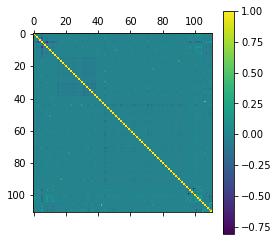
\includegraphics[width=0.45\textwidth]{correlation.png}
\caption{Correlation Plot}
\label{fig:mesh1}
\end{figure}
\end{center}
Looking at the correlation plot in Fig 2, we noticed that there aren't many pairs of features with large values of correlation coefficients. So the possibility of removing one out of a pair of highly correlated features is eliminated. 
Instead we obtained the values of correlation of each feature against case status. We then proceeded to remove those columns which had a correlation values less than 0.007. This removed 55 columns.

\paragraph{\textbf{PCA}}
We now had 56 columns remaining. We attempted to reduce the dimensionality further by applying PCA, which is a dimensionality reduction technique which converts a set of observations of possibly correlated variables or features into a set of values of linearly uncorrelated variables called principal components.
The following is the explained variance obtained against different values of number of principal components.
\begin{center}
\captionof{table}{PCA Results} \label{tab:title}
  \begin{tabularx}{0.367\textwidth}{| c | c |}
  \hline
  \centering
     \ No of Components & \ Explained Variance\\ \hline
	25	& 53.5489\% \\
    30	& 63.1431\% \\
    35	& 72.6216\% \\
    40	& 81.9514\% \\
    45	& 90.574\%  \\
    50	& 97.7323\% \\
    \hline
  \end{tabularx}
  \end{center}
Based on the obtained explained variance values, we chose to reduce the dimensionality to 40 columns as this gave us the desired reduction in the number of columns while also maintaining a minimum explained variance of about 82\%.

\subsubsection{\textbf{Oversampling}}
A challenge with respect to prediction of visa status pertaining to the working data at hand is the fact that the number of visa applicants accepted to those denied is a highly skewed ratio.

\begin{center}
  \begin{tabularx}{0.19\textwidth}{| l | r| }
  \hline
  \centering
     # Denied &
    # Accepted\\ \hline
    5021 & 145752 \\ \hline
  \end{tabularx}
  \end{center}

This indicates that if the current data was split into train and testing dataset, 'Denied' would be underrepresented. The model would output fairly high validation accuracy which may indicate a sophisticated model, but it is in-fact, just labelling each data point in the testing data as "Accepted". \\
In order to work around this problem, we split the dataset into testing and training and over sample the training data on 'Denied'. After choosing the oversampling algorithm \cite{oversample}, the ratio between the two outcomes in the training data is 1:1.

\begin{center}
  \begin{tabularx}{0.19\textwidth}{| l | r| }
  \hline
  \centering
     # Denied &
    # Accepted\\ \hline
    116572 & 116572 \\ \hline
    
  \end{tabularx}
  \end{center}

\subsection{\textbf{Classification Modelling}}
\subsubsection{\textbf{Comparison of Classifiers}}
There exist many different classifications methods to choose from, while trying to predict a class of outcome. Each of these classification techniques perform differently under different situations. We do a comparative analysis to discern the nuances and use the right model for the problem at hand.

\paragraph{\textbf{Neural Networks}}
A neural network is a simplified model of the the human brain. There are typically three parts in a neural network: an input layer, with units representing the input fields; one or more hidden layers; and an output layer, with a unit or units representing the target fields. The units are connected with varying connection strengths. 
The neural network model consists of 3 hidden layers. The model uses 'Sigmoid' as the activation function. It is validated by using binary crossentropy and accuracy as metrics. The net is run for 30 epochs with a batch size of 100.

\paragraph{\textbf{Logistic Regression}}
Logistic regression is the suitable for analysis when the dependent variable is dichotomous. Math behind logistic regression:
\[l = \beta_0 + \beta_1*x_1\]Where l is log-odds, logistic regression was opted for the comparative analysis study because of various of reasons. The output is a probability that the given input point belongs to a certain class.

\paragraph{\textbf{K - Nearest Neighbour}}
KNN can be used for both classification and regression predictive problems. It is a non-parametric, i.e it does not make any assumptions on the underlying data distribution. Due to this property it’s pretty useful in the "real world". The model uses the data of 5 nearest neighbours to predict the case status of the applicant.

\paragraph{\textbf{Decision Trees}}
Decision trees implicitly perform a variable screening of various features to fit the data in the best way possible. This was the key reason why Decision Tress were used for classification. Gini index is used as a hyperparameter for the decision trees.

\paragraph{\textbf{Naive Bayes}}
Naive Bayes classifiers are a collection of classification algorithms based on Bayes’ Theorem. Given a hypothesis 'H'  and evidence 'E', Bayes' theorem states that the relationship between the probability of the hypothesis before getting the evidence  and the probability of the hypothesis after getting the evidence \textit{P(H|E)} is:\\
\begin{equation}
P(H|E) = \frac{P(E|H)P(H)}{P(E)}
\end{equation}
\\
\section{Results and Discussion}
\subsection{\textbf{Comparison of Classifiers}}

\subsubsection{\textbf{k-fold Valdiation Results}}
\begin{center}
\begin{figure}[h]
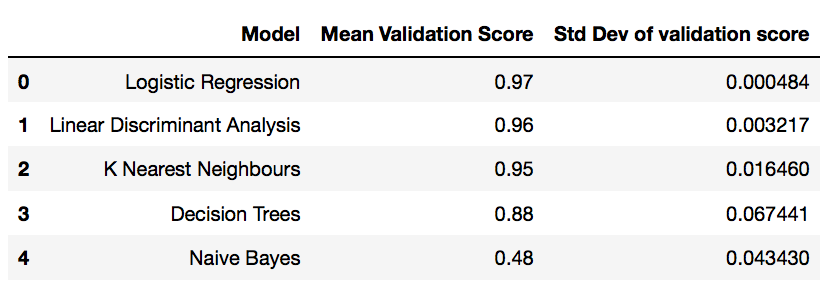
\includegraphics[width=0.45\textwidth]{validation.png}
\caption{Validation Results}
\label{fig:mesh1}
\end{figure}
\end{center}

\subsubsection{\textbf{Test Case Results}}
\begin{center}
\begin{figure}[h]
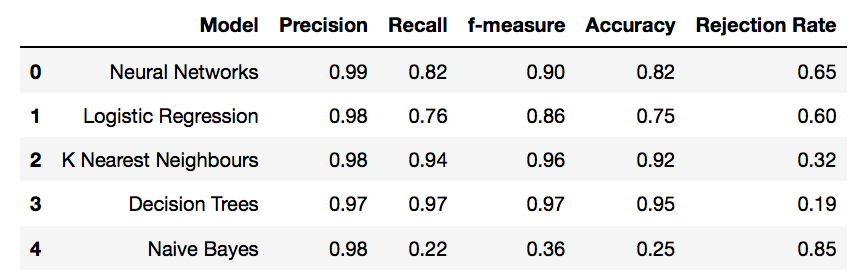
\includegraphics[width=0.45\textwidth]{test.png}
\caption{Test Case Results}
\label{fig:mesh1}
\end{figure}
\end{center}
All the classfiers give very high accuracies due to the fact that the testing sample is imbalanced. Owing to this, accuracy, precision and F-measure are not very good metrics to evaluate the model.
The three classifiers that stand out in this comparative analysis are Neural Networks, Decision Trees and Naive Bayes. All of them have high precision but they have drastically different results for recall and rejection rate. We further look at the Receiver Operating Characteristic (ROC) and the Area Under the Curve (AUC) for these two models to conclude on our working model. 
\\
\paragraph{\textbf{Decision Trees}}

Decision Trees perform the best Recall-wise but it fail when it comes to rejecting values that must be rejected. They have an extremely low rejection rate. The dataset contains more accepted applicants than rejected ones. Therefore, one of the main challenges is to not let this affect the predictive capability of the model. The tree, as the results show, is tuned to classify the majority class very accurately but not the minority class. This poses a problem to the overall prediction capabilities of the algorithm. The AUC metric also indicates that the tree does not do a good job of separating the two classes. With these results, we infer that Decision Tree is not suitable to tackle our classification.
\begin{figure}[h]%
    \centering
    \subfloat[Confusion Matrix]{{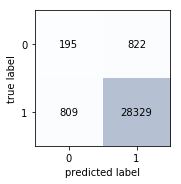
\includegraphics[width=0.15\textwidth]{dt.png} }}%
    \qquad
    \subfloat[ROC Curve]{{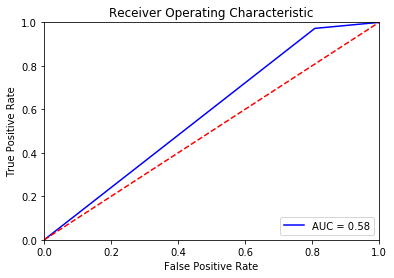
\includegraphics[width=0.27\textwidth]{dt-aoc.png}}}%
    \caption{Decision Trees}%
    \label{fig:}%
\end{figure}
\\
\paragraph{\textbf{Naive Bayes}}
Contrasting the results of that of Decision Trees is Naive Bayes. They have the highest rejection rate among all the classifiers but a low recall. 
This means they perform very well on the minority samples but not on the majority samples. Similar to the Decision Tree, its AUC is low which means it does not separate the two classes well. This model too is not suitable for use. 
\begin{figure}[h]%
    \centering
    \subfloat[Confusion Matrix]{{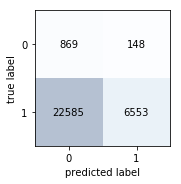
\includegraphics[width=0.15\textwidth]{nb.png} }}%
    \qquad
    \subfloat[ROC Curve]{{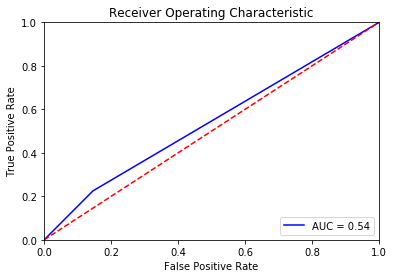
\includegraphics[width=0.27\textwidth]{nb-aoc.png}}}%
    \caption{Naive Bayes}%
    \label{fig:}%
\end{figure}
\\
\paragraph{\textbf{Neural Networks}}
The Area Under the Curve (AUC) of Neural Networks is 0.7 which means it separates the classes fairly well when compared to a random classifier. AUC is the average of the classifier accuracy over all possible thresholds between 0 and 1. Whereas Accuracy of a model is typically based on a '0.5' threshold. 
Neural Networks have a very high rejection rate which means out of all the samples that had to be rejected most of them were indeed rejected. It also has a high recall rate, which means it is classifying 'Accepted' values correctly a lot of the times. This validates the fact that the Net handles the majority as well as the minority case. 
\begin{figure}[h]%
    \centering
    \subfloat[Confusion Matrix]{{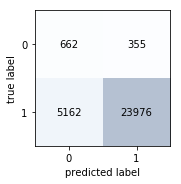
\includegraphics[width=0.15\textwidth]{nn.png} }}%
    \qquad
    \subfloat[ROC Curve]{{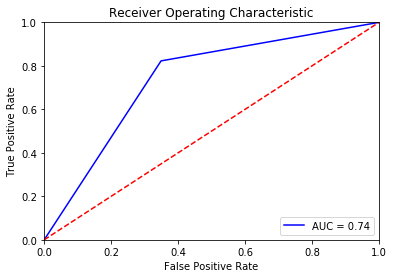
\includegraphics[width=0.27\textwidth]{nn-aoc.png} }}%
    \caption{Neural Networks}%
    \label{fig:}%
\end{figure}
\subsection{\textbf{Analysis of Neural Network results using K-Nearest Neighbours}}
From Fig 7 (test case results), K- Nearest Neighbour appears to have the highest accuracy metrics overall with the exception of reject rate. This can be exploited to gain insights into the impact of attributes on the outcome. We locate the five nearest neighbours by computing the distance between two applications using the K-Nearest Neighbour algorithm \cite{KNN}. Once we got these results, we arrived at the most distinguishing attributes between neighbours of different case status outcomes. It was found that 'foreign\_worker\_info\_inst', 'wage\_offer\_from\_9089','foreign\_worker\_info\_major' and 'agent\_firm\_name' are the top attributes that separate two neighbours with different application status outcomes but otherwise similar features.
\begin{center}
\begin{figure}[h]
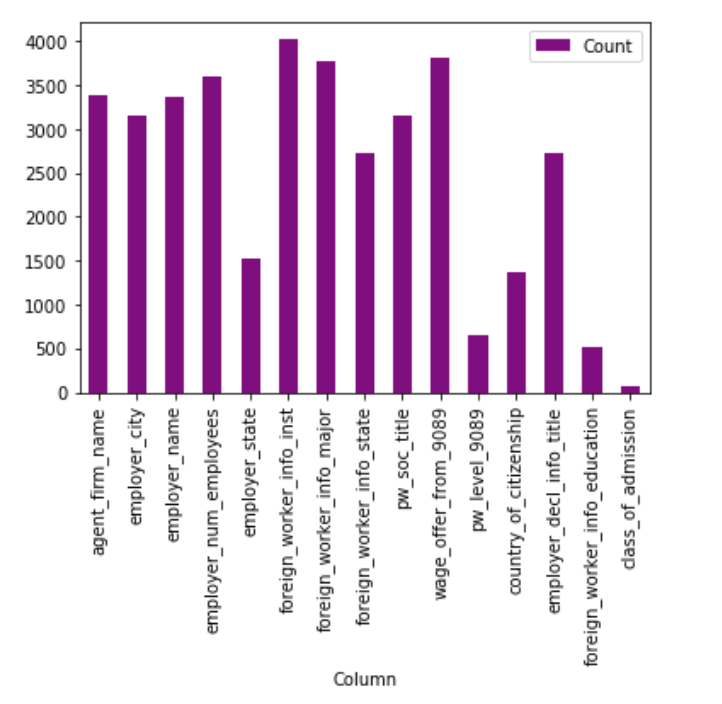
\includegraphics[width=0.45\textwidth]{rec.png}
\caption{Plot of Distinguishing Attributes}
\label{fig:mesh1}
\end{figure}
\end{center}
\section{Conclusions}
Processing visa applications has historically been purely human based. There has been little to no involvement of machine learning models to aid the process. We attempted to try to make a machine process a visa application and  were presented with interesting conclusions.

Neural Networks provide the most suitable predictive capabilities required for our dataset which is high recall and high reject-rate. They correlate seemingly uncorrelated attributes by creating connections similar to that of human neurons. Neural networks have a better ability to explain complex non linear relationships which could explain the superior results of this model.

Future work can include working on a dataset that is more balanced and has a roughly equal number of rejected and certified applications in order to eliminate the need for over sampling. While over sampling is a valid technique for generation of balanced datasets, it provides a less accurate representation of the population.

A visa application that was certified a year ago may not be certified today. This is due to the dynamically changing factors like political climate, immigration policies etc. Our future work can aim towards including these variables to generate a more accurate result.

\section{Contribution}
\subsection{\textbf{Dweepa}}
\begin{itemize}
  \item Processing categorical features and bringing down the number of unique values of these columns.
  \item Performing a comparative analysis of different classifiers with and without oversampling on the working dataset.
  \item Analyzing results and determining the features with a high impact using K nearest Neighbour.
\end{itemize}
\subsection{\textbf{Kavya}}
\begin{itemize}
  \item Initial pre-processing and standardization of features
  \item Dimensionality reduction through correlation plots and PCA
  \item Generating classifiers for L1 and F1 visa types
\end{itemize}
\subsection{\textbf{Ishita}}
\begin{itemize}
  \item Reduction of dataset and imputation of null values
  \item Encoding categorical variables using one hot and label encoding
  \item Generating classifiers for H1B visa type
\end{itemize}



\begin{thebibliography}{00}
\bibitem{berk} Nihar Dalmia et. Al: \textit{\url{https://www.ischool.berkeley.edu/sites/default/files/sproject\_attachments/\\aml\_project\_report.pdf}}
\bibitem{stanford} Beliz Gunel, Onur Cezmi Mutlu: \textit{\url{http://cs229.stanford.edu/proj2017/final-reports/5208701.pdf}}
\bibitem{github} Jinglin Li, H1-B Visa Prediciton: \textit{\url{https://github.com/Jinglin-LI/H1B-Visa-Prediction-by-Machine-Learning-Algorithm}}
\bibitem{dataset} 
Dataset:  \textit{\url{https://www.kaggle.com/jboysen/us-perm-visas/kernels}}
\bibitem{tfidf}
TFIDFVectorizer: \textit{\url{https://scikit-learn.org/stable/modules/generated/sklearn.feature_extraction.text.TfidfVectorizer.html}}
\bibitem{kmeans}
Kmeans Algorithm: \textit{\url{https://scikit-learn.org/stable/modules/generated/sklearn.cluster.KMeans.html}}
\bibitem{oversample}
Random Oversampling Algorithm: \textit{\url{https://imbalanced-learn.org/en/stable/over_sampling.html}}
\bibitem{KNN}
K-Nearest Neighbour Algorithm: \textit{}
\end{thebibliography}
\vspace{12pt}
\end{document}
